\documentclass[a4paper,12pt]{article}
\usepackage[left=2cm,right=2cm,top=2cm,bottom=2cm]{geometry} % Do ustawień marginesów
\usepackage{multicol} % Dla podziału na kolumny
\usepackage{ragged2e} % Dla justowania tekstu
\usepackage{graphicx} % Required for inserting images
\usepackage{float}
\usepackage{caption}
\usepackage{amsmath} % Math formulas
\usepackage{amssymb} % Symbols
\usepackage[svgnames]{xcolor}
\usepackage[colorlinks=true, urlcolor=blue, linkcolor=black, citecolor=orange]{hyperref} % Hyperlinks
\usepackage{polski} % Polish language
\usepackage[utf8]{inputenc} % Text encoding
\usepackage{enumitem} % Pakiet do elastycznego sterowania listami
\usepackage{indentfirst}
\usepackage{array}

\begin{document}

% Górna część strony
\noindent
\begin{minipage}{0.5\textwidth}
    \raggedright
    \textbf{Piotr Durniat} \\
    I rok, Fizyka \\
    Wtorek, 8:00-10:15 \\
    \vspace{0.5cm}
    \vspace{0.5cm}
\end{minipage}%
\begin{minipage}{0.5\textwidth}
    \raggedleft
    Data wykonania pomiarów: \\
    18.03.2025 \\
    \vspace{0.5cm}
    Prowadząca: \\
    dr Iwona Mróz
\end{minipage}

% ------------------------------------------------------------

% Tytuł ćwiczenia
\vspace{2cm}
\begin{center}
    \LARGE \textbf{Ćwiczenie nr 11} \\[0.5cm]
    \Large \textbf{Wyznaczanie elipsoidy bezwładności bryły sztywnej}
\end{center}

\vspace{1cm}
\noindent

\tableofcontents
\newpage


% ------------------------------------------------------------

% --------- WSTĘP TEORETYCZNY ---------
\section{Wstęp teoretyczny}

\subsection*{Pierwsza zasada dynamiki ruchu obrotowego}

Pierwsza zasada dynamiki ruchu obrotowego stwierdza, że jeżeli na ciało nie działa wypadkowy moment siły, to ciało pozostaje w spoczynku lub porusza się ruchem obrotowym jednostajnym. Matematycznie można to zapisać jako:

\begin{equation*}
    \sum_{i=1}^{n} M_i = 0
    \Rightarrow
    \frac{d\vec{L}}{dt} = 0
\end{equation*}

gdzie $M_i$ oznacza $i$-ty moment siły działający na ciało, a $\vec{L}$ to moment pędu ciała. Moment pędu wyraża się wzorem:

\begin{equation*}
    \vec{L} = I\vec{\omega}
\end{equation*}

gdzie $I$ oznacza moment bezwładności ciała, a $\vec{\omega}$ jego prędkość kątową.

\subsection*{Tensor momentu bezwładności}

Moment bezwładności ciała zależy od wyboru osi obrotu. Do pełnego opisu własności bezwładnościowych ciała służy tensor momentu bezwładności, który ma postać macierzy:

\begin{equation*}
    I = \begin{pmatrix}
        I_{xx} & I_{xy} & I_{xz} \\
        I_{yx} & I_{yy} & I_{yz} \\
        I_{zx} & I_{zy} & I_{zz}
    \end{pmatrix}
\end{equation*}

Elementy tego tensora definiuje się następująco:

\begin{equation*}
    I_{ij} = \sum_{k=1}^{n} m_k (r_{k}^2\delta_{ij} - r_{ki}r_{kj})
\end{equation*}

gdzie $m_k$ oznacza masę $k$-tego elementu ciała, $r_{ki}$ to współrzędna $k$-tego elementu na osi $i$, a $\delta_{ij}$ to delta Kroneckera.

\subsection*{Elipsoida bezwładności}

Elipsoida bezwładności to powierzchnia, której odległość $r$ od środka masy w dowolnym kierunku jest powiązana z momentem bezwładności $I$ względem tej osi zależnością:

\begin{equation*}
    I = \frac{1}{r^2}
\end{equation*}

Długości półosi elipsoidy są równe odwrotnościom pierwiastków kwadratowych z głównych momentów bezwładności:

\begin{equation*}
    a = \frac{1}{\sqrt{I_{xx}}}, \quad
    b = \frac{1}{\sqrt{I_{yy}}}, \quad
    c = \frac{1}{\sqrt{I_{zz}}}
\end{equation*}

Znajomość elipsoidy bezwładności umożliwia wyznaczenie momentu bezwładności dla dowolnej osi obrotu.

\subsection*{Wahadło torsyjne}

Wahadło torsyjne to układ składający się z pręta zawieszonego na nici, który może wykonywać drgania skrętne. Po wychyleniu o kąt $\theta$ od położenia równowagi, na pręt działa moment siły sprężystości $M$:

\begin{equation}
    M = -k\theta
\end{equation}

gdzie $k$ jest współczynnikiem sprężystości skrętnej. Okres drgań wahadła torsyjnego wyraża się wzorem:

\begin{equation} \label{eq:okres_drgan_w_zaleznosci_od_momentu_bezwladnosci}
    T = 2\pi \sqrt{\frac{I}{k}}
\end{equation}

gdzie:
\begin{itemize}
    \item $I$ -- moment bezwładności bryły
    \item $k$ -- moment kierujący wahadła
\end{itemize}

Z powyższego wzoru można wyznaczyć moment bezwładności:

\begin{equation} \label{eq:moment_bezwladnosci_w_zaleznosci_od_okresu}
    I = k \left(\frac{T}{2\pi}\right)^2
\end{equation}

Wstęp teoretyczny opracowano na podstawie podręcznika \cite{Drynski1976} (rozdział 19) oraz instrukcji do ćwiczenia \cite{lab11manual}.
% --------- OPIS DOŚWIADCZENIA ---------
\section{Opis doświadczenia}

Celem doświadczenia było wyznaczenie elipsoidy bezwładności bryły sztywnej metodą wahadła torsyjnego. Pomiary wykonano w następujących etapach:

\begin{enumerate}
    \item \textbf{Pomiar okresu drgań samej ramki} \\
          Zmierzono czas trwania 10 drgań pustej ramki wahadła torsyjnego ($T_0$). Ramkę wychylano o ustalony kąt za pomocą elektromagnesu, a po jego wyłączeniu mierzono czas drgań układem elektronicznym.

    \item \textbf{Pomiar okresu drgań z bryłą wzorcową} \\
          Wykonano pomiar czasu 10 drgań ramki z zamocowanym walcem wzorcowym o masie 1330 g ($T_w$). Zmierzono również wymiary walca niezbędne do obliczenia jego momentu bezwładności.

    \item \textbf{Pomiary dla badanej bryły} \\
          Dla badanej bryły wykonano serię pomiarów czasu 10 drgań ($T_1$):
          \begin{itemize}
              \item względem trzech osi głównych przechodzących przez środek masy
              \item względem jednej dowolnie wybranej osi przechodzącej przez środek masy
              \item względem osi wskazanej przez prowadzącego, nieprzechodzącej przez środek masy
          \end{itemize}
\end{enumerate}

Układ pomiarowy składał się z wahadła torsyjnego z elektromagnetycznym mechanizmem wyzwalania drgań oraz elektronicznego układu pomiaru czasu.

\section{Opracowanie wyników pomiarów}

% ---------- TABELE ----------
\subsection{Tabele pomiarowe}

\begin{itemize}
    \item Błąd wskazania zerowego suwmiarki wyniósł 0.15 mm.
    \item Niepewność wzorcowania suwmiarki $\Delta_d D = 0.05$ mm.
    \item Kąt $\alpha = 30^\circ$.
\end{itemize}

\begin{table}[H]
    \centering
    \begin{tabular}{|l|c|c|}
        \hline
        \textbf{Rodzaj układu} & \textbf{Czas 10 drgań [s]} & \textbf{Okres T [s]} \\
        \hline
        Sama ramka & 18.135 & 1.8135 \\
        \hline
        Ramka + walec wzorcowy & 25.192 & 2.5192 \\
        \hline
    \end{tabular}
    \caption{Pomiar czasu drgań ramki i ramki z walcem wzorcowym}
    \label{tab:pomiar_czasu_drgan_ramki_z_walcem}
\end{table}

\begin{table}[H]
    \centering
    \begin{tabular}{|l|c|c|}
        \hline
        \textbf{Oś obrotu} & \textbf{Czas 10 drgań [s]} & \textbf{Okres T [s]} \\
        \hline
        Główna oś 1 (x) & 23.001 & 2.3001 \\
        \hline
        Główna oś 2 (y) & 23.008 & 2.3008 \\
        \hline
        Główna oś 3 (z) & 22.937 & 2.2937 \\
        \hline
        Dowolna oś przez środek masy (s) & 23.006 & 2.3006 \\
        \hline
        Dowolna oś nieprzechodząca przez środek masy (t) & 22.573 & 2.2573 \\
        \hline
    \end{tabular}
    \caption{Pomiar czasu drgań ramki z badaną bryłą dla różnych osi}
    \label{tab:pomiar_czasu_drgan_badanej_bryly}
\end{table}

\begin{table}[H]
    \centering
    \begin{tabular}{|l|c|c|}
        \hline
        \textbf{Wielkość} & \textbf{Wartość [mm]} & \textbf{Po korekcie [mm]} \\
        \hline
        Średnica podstawy $d$ [mm] & 60.15 & 60.00 \\
        \hline
        Wysokość walca $h$ [mm] & 60.15 & 60.00\\
        \hline
        Masa walca $m$ [g] & 1330 & 1330 \\
        \hline
    \end{tabular}
    \caption{Rozmiary bryły wzorcowej, wraz z korektą wskazania zerowego}
    \label{tab:rozmiar_bryly_wzorcowej}
\end{table}

% ---------- OBLICZENIA ----------
\subsection{Moment bezwładności bryły wzorcowej}

Badaną bryłą jest walec o wymiarach w tabeli \ref{tab:rozmiar_bryly_wzorcowej}, moment bezwładności walca dla osi przechodzącej przez środki podstaw określa wzór:

\begin{equation} \label{eq:moment_bezwladnosci_walca}
    I_w = \frac{1}{2}mr^2 = \frac{1}{2}m\left(\frac{d}{2}\right)^2
\end{equation}

Podstawiając dane z tabeli \ref{tab:rozmiar_bryly_wzorcowej} otrzymujemy:

\begin{equation} \label{eq:moment_bezwladnosci_walca_wartosc}
    I_w = \frac{1}{2} \cdot 1,330 \cdot \left(\frac{0.06}{2}\right)^2 = 0.0005985\,\text{kgm}^2
\end{equation}


\subsection{Moment bezwładności badanej bryły} \label{sec:moment_bezwladnosci_badanej_bryly}

Dla samej ramki okres drgań na podstawie wzoru \ref{eq:okres_drgan_w_zaleznosci_od_momentu_bezwladnosci} wynosi:

\begin{equation} \label{eq:okres_drgan_ramki}
    T_0 = 2\pi \sqrt{\frac{I_0}{k}}
\end{equation}

Stąd okres $T_w$ drgań ramki z bryłą wzorcową o momencie bezwładności $I_w$ wynosi:

\begin{equation} \label{eq:okres_drgan_ramki_z_walcem}
    T_w = 2\pi \sqrt{\frac{I_0 + I_w}{k}}
\end{equation}

Zatem z równań \eqref{eq:okres_drgan_ramki} i \eqref{eq:okres_drgan_ramki_z_walcem} moment kierujący wahadła wynosi:

\begin{equation} \label{eq:moment_kierujacy_w_zaleznosci_od_okresu}
    k = \frac{4\pi^2 I_w}{T_w^2 - T_0^2}
\end{equation}

Z wzorów \eqref{eq:moment_bezwladnosci_w_zaleznosci_od_okresu} i \eqref{eq:moment_kierujacy_w_zaleznosci_od_okresu} otrzymujemy moment bezwładności $I_x$ badanej bryły:

\begin{equation} \label{eq:moment_bezwladnosci_badanej_bryly}
    I_x = \frac{T_x^2 - T_0^2}{T_w^2 - T_0^2} \cdot I_w
\end{equation}

Po podstawieniu okresów drgań z tabel \ref{tab:pomiar_czasu_drgan_badanej_bryly} oraz \ref{tab:pomiar_czasu_drgan_ramki_z_walcem} i momentu bezwładności walca $I_w$ z wzoru \eqref{eq:moment_bezwladnosci_walca_wartosc} otrzymujemy (moment oznaczony jako $I_{[x]}$ oznacza moment osi oznaczonej jako $[x]$ w tabeli~\ref{tab:pomiar_czasu_drgan_badanej_bryly}):

\begin{table}[H]
    \centering
    \begin{tabular}{|c|c|}
        \hline
        Oś & Moment bezwładności [$\text{kg}\cdot\text{m}^2$] \\
        \hline
        $I_x$ & 0,000392 \\
        $I_y$ & 0,000392 \\
        $I_z$ & 0,000386 \\
        $I_s$ & 0,000392 \\
        $I_t$ & 0,000354 \\
        \hline
    \end{tabular}
    \caption{Momenty bezwładności względem poszczególnych osi}
    \label{tab:momenty_bezwladnosci}
\end{table}

Przykładowe obliczenia dla $I_x$:

\begin{equation*}
    I_x = \frac{(2,3001)^2 - (1,8135)^2}{(2,5192)^2 - (1,8135)^2} \cdot 0,0005985 = 0,000392\,\text{kgm}^2
\end{equation*}


% 2. Obliczyć momenty bezwładności badanej bryły względem wszystkich osi obrotu, dla których mierzono T1.

\subsection{Wyznaczanie elipsoidy bezwładności badanej bryły}


Równanie elipsoidy ma postać:

\begin{equation} \label{eq:elipsoida_bezwladnosci}
    \frac{x^2}{a^2} + \frac{y^2}{b^2} + \frac{z^2}{c^2} = 1
\end{equation}

a, b, c to półosie elipsoidy, które są zdefiniowane jako:

\begin{equation*}
    a = \frac{1}{\sqrt{I_x}}, \quad
    b = \frac{1}{\sqrt{I_y}}, \quad
    c = \frac{1}{\sqrt{I_z}}
\end{equation*}

Podstawiając momenty bezwładności z tabeli \ref{tab:momenty_bezwladnosci} otrzymujemy:

\begin{equation*}
    a=50,519636 \text{m} \quad
    b=50,479042 \text{m} \quad
    c=50,894785 \text{m}
\end{equation*}

\subsection{Wyznaczanie momentu bezwładności względem osi niebędących głównymi osiami bezwładności}

% 4. Wyznaczyć długość odcinka Ri łączącego początek układu współrzędnych z punktem przebicia P elipsoidy bezwładności przez wskazaną przez prowadzącego oś, nie będącą osią główną. Na tej podstawie obliczyć moment bezwładności bryły względem tej osi.

% My tu chyba mamy dla obydu osi to zrobić (nieprzechodząca przez środek masy i przechodząca przez środek masy)
\subsubsection{Oś przechodząca przez środek masy (s)}

Znając momenty bezwładności względem głównych osi możemy obliczyć momenty bezwładności względem osi niebędących głównymi osiami bezwładności, korzystając z wzoru:

\begin{equation} \label{eq:moment_bezwladnosci_elipsoida}
    I_i = \frac{1}{R_i^2}
\end{equation}

gdzie $R_i$ to odległość między początkiem układu współrzędnych a punktem przebicia elipsoidy bezwładności przez wybraną oś:

\begin{equation} \label{eq:odleglosc_od_srodka_masy_do_punktu_przebicia_osi}
    R_i = \sqrt{x^2 + y^2 + z^2}
\end{equation}

Wybrana oś przechodzi przez dwa przeciwległe wierzchołki sześcianu o boku $a$, stąd współrzędne jednego z punktów leżącego na osi $s$ wynoszą:

\begin{equation*}
    x = \frac{a}{2}, \quad
    y = \frac{a}{2}, \quad
    z = \frac{a}{2}
\end{equation*}

Równanie prostej przechodzącej przez środek sześcianu (0, 0, 0) i punkt (a/2, a/2, a/2) ma postać:

\begin{align} \label{eq:prosta_przechodzaca_przez_srodek_szesciany}
    \frac{x}{a/2} = \frac{y}{a/2} = \frac{z}{a/2}
    \Rightarrow
    x = y = z
\end{align}

Tworzymy układ równań \eqref{eq:elipsoida_bezwladnosci} i \eqref{eq:prosta_przechodzaca_przez_srodek_szesciany} i rozwiązujemy go względem $x$, $y$, $z$:

\begin{align*} \label{eq:rozwiazanie_ukladu_rownan}
     & \begin{cases}
           \frac{x^2}{a^2} + \frac{y^2}{b^2} + \frac{z^2}{c^2}  = 1 \\
           x = y = z
       \end{cases} \\
     & \frac{x^2}{a^2} + \frac{x^2}{b^2} + \frac{x^2}{c^2} = 1              \\
     & x^2 \left( \frac{1}{a^2} + \frac{1}{b^2} + \frac{1}{c^2} \right) = 1 \\
     & x^2 = \frac{1}{\frac{1}{a^2} + \frac{1}{b^2} + \frac{1}{c^2}}        \\
     & x = \sqrt{\frac{1}{\frac{1}{a^2} + \frac{1}{b^2} + \frac{1}{c^2}}}
\end{align*}

Podstawiając wartości $a$, $b$, $c$ otrzymujemy:

\begin{equation*}
    x = y = z = \sqrt{\frac{1}{\frac{1}{50,519636^2} + \frac{1}{50,479042^2} + \frac{1}{50,894785^2}}} = 29.2313\,\text{m}
\end{equation*}

Stąd podstawiając do wzoru \eqref{eq:moment_bezwladnosci_elipsoida} otrzymujemy:

\begin{align*}
    I_{s, elip} & = \frac{1}{R_i^2} = \frac{1}{(\sqrt{x^2 + y^2 + z^2})^2}  = \frac{1}{3x^2} \\
                & = \frac{1}{ 3 \cdot 29.231314^2} = 0.0003901\,\text{kgm}^2
\end{align*}

\subsubsection{Oś nieprzechodząca przez środek masy (t)}

Wybrana oś przechodzi przez jeden wybrany wierzchołek sześcianu oraz środek krawędzi przeciwległej, stąd wyznaczone zostały dwa punkty przez które przechodzi oś $t$ (rys. \ref{fig:cube}).

\begin{figure}[H]
    \centering
    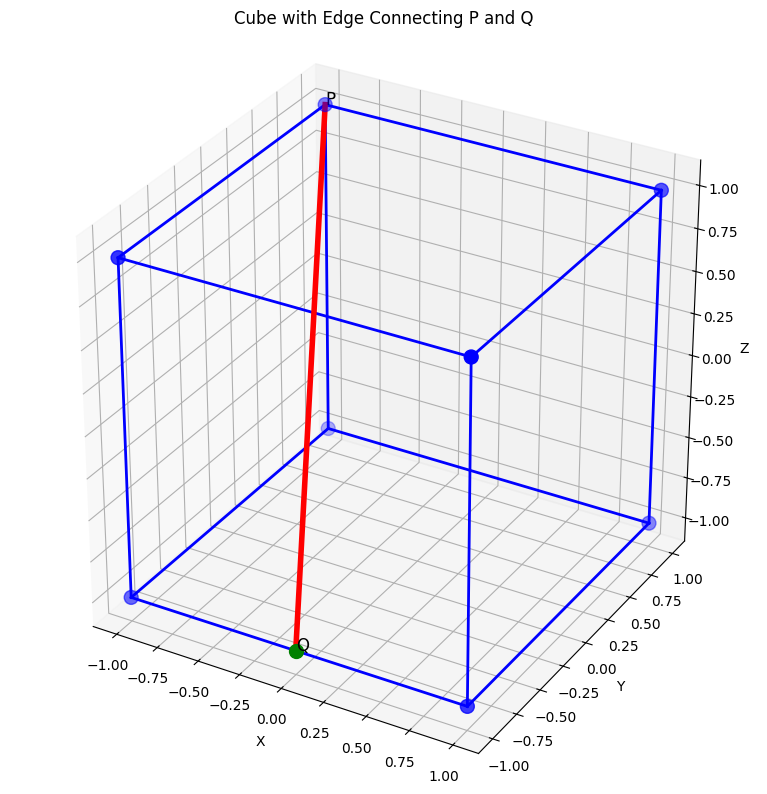
\includegraphics[width=0.5\textwidth]{cube.png}
    \caption{Sześcian z zaznaczoną osią $t$ przechodzącą przez wierzchołek i środek przeciwległej krawędzi}
    \label{fig:cube}
\end{figure}



\begin{align*}
    \vec{P} & = (\frac{-a}{2}, \frac{a}{2}, \frac{a}{2}) \\
    \vec{Q} & = (0, -\frac{a}{2}, -\frac{a}{2})
\end{align*}

Wektor kierunkowy osi $t$ to:

$$
    \vec{t} = \vec{Q} - \vec{P} = (0, -\frac{a}{2}, -\frac{a}{2}) - (\frac{-a}{2}, \frac{a}{2}, \frac{a}{2}) = (\frac{a}{2}, -a, -a)
$$


Wyznaczamy oś $t'$ równoległą do osi $t$ przechodzącą przez środek sześcianu (0, 0, 0):

$$
    t' = (0, 0, 0) + \vec{t} = (\frac{a}{2}, -a, -a)
$$



Równanie prostej $t'$ przechodzącej przez środek sześcianu (0, 0, 0) o zwrocie wskazanym przez wektor kierunkowy $\vec{t}$ to:

$$
    \begin{cases}
        x = s(\frac{a}{2}) \\
        y = s(-a)          \\
        z = s(-a)
    \end{cases}
$$

w postaci kanonicznej:

\begin{align*}
     & \frac{x}{\frac{a}{2}} = \frac{y}{-a} = \frac{z}{-a}    \\
     & \Rightarrow                                            \\
     & \frac{2x}{a} = \frac{y}{-a} = \frac{z}{-a} / \cdot (a) \\
     & 2x = -y = -z
\end{align*}

Punkt przebicia elipsoidy bezwładności z osią $t'$ obliczamy, rozwiązując układ równań \eqref{eq:elipsoida_bezwladnosci} i \eqref{eq:prosta_przechodzaca_przez_srodek_szesciany}:



$$
    \begin{cases}
        \frac{x^2}{a^2} + \frac{y^2}{b^2} + \frac{z^2}{c^2} = 1 \\
        2x = -y = -z
    \end{cases}
$$


Rozwiązanie układu równań:


\[
    \begin{cases}
        x = \pm\frac{1}{\sqrt{\frac{1}{a^2} + \frac{4}{b^2} + \frac{4}{c^2}}}  \\
        y = \mp2\frac{1}{\sqrt{\frac{1}{a^2} + \frac{4}{b^2} + \frac{4}{c^2}}} \\
        z = \mp2\frac{1}{\sqrt{\frac{1}{a^2} + \frac{4}{b^2} + \frac{4}{c^2}}}
    \end{cases}
\]

Wybierając jeden z dwóch punktów:


\[
    \begin{cases}
        x = +\frac{1}{\sqrt{\frac{1}{a^2} + \frac{4}{b^2} + \frac{4}{c^2}}}  \\
        y = -2\frac{1}{\sqrt{\frac{1}{a^2} + \frac{4}{b^2} + \frac{4}{c^2}}} \\
        z = -2\frac{1}{\sqrt{\frac{1}{a^2} + \frac{4}{b^2} + \frac{4}{c^2}}}
    \end{cases}
\]

Podstawiając wartości $a$, $b$, $c$ otrzymujemy:


% \begin{verbatim}
%     a = 50.51963556001976;
%     b = 50.47904236866827;
%     c = 50.89478538917224;

%     x = 1 / Sqrt[1/a^2 + 4/b^2 + 4/c^2];
%     y = -2 / Sqrt[1/a^2 + 4/b^2 + 4/c^2];
%     z = -2 / Sqrt[1/a^2 + 4/b^2 + 4/c^2];
% \end{verbatim}

% \begin{verbatim}
%     {x, y, z} = {16.889036632620389, -33.77807326524078, -33.77807326524078}
% \end{verbatim}


\begin{equation*}
    \begin{cases}
        x \approx 16.89\text{ m}  \\
        y \approx -33.78\text{ m} \\
        z \approx -33.78\text{ m}
    \end{cases}
\end{equation*}



Moment bezwładności względem osi $t$ obliczamy z wzoru:
\[
    I_t = \frac{1}{x^2 + y^2 + z^2}
\]
gdzie:
\begin{align*}
    x & = 16.889036632620389 \\
    y & = -33.77807326524078 \\
    z & = -33.77807326524078
\end{align*}

Podstawiając wartości $x$, $y$ i $z$:
\begin{align*}
    I_t & = \frac{1}{(16.8890)^2 + (-33.7780)^2 + (-33.7780)^2} \\
        & = \frac{1}{285.2397 + 1140.9588 + 1140.9588}          \\
        & = \frac{1}{2567.1573}                                 \\
        & \approx 0.0003895
\end{align*}

Zatem moment bezwładności względem osi $t'$ wynosi około $0.0003895\,\text{kgm}^2$.\par
Aby obliczyć moment bezwładności względem osi $t$ należy zastosować twierdzenie Steinera\par
\subsubsection*{Obliczenie odległości między osiami $t$ i $t'$}

Oś $t$ przechodzi przez punkty $P = \left(\frac{-a}{2}, \frac{a}{2}, \frac{a}{2}\right)$ oraz $Q = \left(0, -\frac{a}{2}, -\frac{a}{2}\right)$.
Oś $t'$ przechodzi przez początek układu współrzędnych $O = (0, 0, 0)$ i jest równoległa do osi $t$.

Wektor kierunkowy osi $t$ oznaczamy jako $\vec{t}$ i obliczamy, odejmując współrzędne punktu $P$ od współrzędnych punktu $Q$:
\[
    \vec{t} = Q - P = \left(0 - \left(\frac{-a}{2}\right), -\frac{a}{2} - \frac{a}{2}, -\frac{a}{2} - \frac{a}{2}\right) = \left(\frac{a}{2}, -a, -a\right)
\]


Wybieramy punkt $P = \left(\frac{-a}{2}, \frac{a}{2}, \frac{a}{2}\right)$, który należy do osi $t$.


Wybieramy punkt $O = (0, 0, 0)$ na osi $t'$. Wektor łączący $P$ z $O$ oznaczamy jako $\vec{v}$ i obliczamy, odejmując współrzędne punktu $P$ od współrzędnych punktu $O$:
\[
    \vec{v} = O - P = \left(0 - \left(\frac{-a}{2}\right), 0 - \frac{a}{2}, 0 - \frac{a}{2}\right) = \left(\frac{a}{2}, -\frac{a}{2}, -\frac{a}{2}\right)
\]


Iloczyn wektorowy $\vec{t} \times \vec{v}$ jest dany przez wyznacznik:
\[
    \vec{t} \times \vec{v} = \begin{vmatrix} \mathbf{i} & \mathbf{j} & \mathbf{k} \\ \frac{a}{2} & -a & -a \\ \frac{a}{2} & -\frac{a}{2} & -\frac{a}{2} \end{vmatrix} = \mathbf{i}((-a)(-\frac{a}{2}) - (-a)(-\frac{a}{2})) - \mathbf{j}((\frac{a}{2})(-\frac{a}{2}) - (-a)(\frac{a}{2})) + \mathbf{k}((\frac{a}{2})(-\frac{a}{2}) - (-a)(\frac{a}{2}))
\]
\[
    = \mathbf{i}\left(\frac{a^2}{2} - \frac{a^2}{2}\right) - \mathbf{j}\left(-\frac{a^2}{4} + \frac{a^2}{2}\right) + \mathbf{k}\left(-\frac{a^2}{4} + \frac{a^2}{2}\right) = 0\mathbf{i} - \frac{a^2}{4}\mathbf{j} + \frac{a^2}{4}\mathbf{k} = \left(0, -\frac{a^2}{4}, \frac{a^2}{4}\right)
\]

Obliczmy masę sześcianu $m$
\[
    m = \frac{6I_x}{a^2}
\]

Podstawiamy wartości:

\[
    m = \frac{6 \cdot 0.000392}{(0.05)^2}
\]


Ostatecznie:

\[
    m \approx 0.941 \text{ kg}
\]


Długość wektora $\vec{t} \times \vec{v}$ jest dana wzorem:
\[
    |\vec{t} \times \vec{v}| = \sqrt{0^2 + \left(-\frac{a^2}{4}\right)^2 + \left(\frac{a^2}{4}\right)^2} = \sqrt{0 + \frac{a^4}{16} + \frac{a^4}{16}} = \sqrt{\frac{2a^4}{16}} = \sqrt{\frac{a^4}{8}} = \frac{a^2}{2\sqrt{2}} = \frac{a^2\sqrt{2}}{4}
\]


Długość wektora kierunkowego $\vec{t}$ jest dana wzorem:
\[
    |\vec{t}| = \sqrt{\left(\frac{a}{2}\right)^2 + (-a)^2 + (-a)^2} = \sqrt{\frac{a^2}{4} + a^2 + a^2} = \sqrt{\frac{a^2}{4} + \frac{4a^2}{4} + \frac{4a^2}{4}} = \sqrt{\frac{9a^2}{4}} = \frac{3|a|}{2}
\]
Ponieważ $a$ jest długością boku sześcianu, jest dodatnie, więc $|\vec{t}| = \frac{3a}{2}$.


Odległość $d$ między prostymi jest równa ilorazowi długości iloczynu wektorowego i długości wektora kierunkowego:
\[
    d = \frac{|\vec{t} \times \vec{v}|}{|\vec{t}|} = \frac{\frac{a^2\sqrt{2}}{4}}{\frac{3a}{2}} = \frac{a^2\sqrt{2}}{4} \times \frac{2}{3a} = \frac{2a^2\sqrt{2}}{12a} = \frac{a\sqrt{2}}{6}
\]

Podstawiając $a = 0.05$, otrzymujemy:
\[
    d = \frac{0.05 \times \sqrt{2}}{6} \approx \frac{0.05 \times 1.4142}{6} \approx \frac{0.07071}{6} \approx 0.011785
\]
Zatem odległość między osiami $t$ i $t'$ wynosi około $0.011785$.\par


Moment bezwładności względem osi $t$ ($I_t$) możemy obliczyć, korzystając z twierdzenia Steinera:
\[
    I_t = I_{t'} + m \cdot d^2
\]
gdzie:
\begin{align*}
    I_{t'} & = 0.00038953 \text{ kgm}^2 \quad \text{(moment bezwładności względem osi } t') \\
    m      & = 0.9408 \text{ kg} \quad \text{(masa bryły)}                                  \\
    d      & = 0.011785 \text{ m} \quad \text{(odległość między osiami } t \text{ i } t')
\end{align*}

Podstawiając te wartości do wzoru:
\[
    I_t = 0.00038953 \text{ kgm}^2 + 0.9408 \text{ kg} \cdot (0.011785 \text{ m})^2
\]

\[
    I_t \approx 0.0005203012 \text{ kgm}^2
\]

Zatem moment bezwładności względem osi $t$ wynosi około $0.0005203$ [$kgm^2$].

\subsubsection*{Moment bezwładności osi $T$ sposób 2}

Ze specyfiki sześcianu dowiadujemy się, że moment bezwładności dowolnej osi przechodzącej przez jego środek masy wyraża się:
\[
    I = \frac{ma^2}{6}
\]
Wiedząc, że oś $t$ przechodzi przez środek, także może zostać wyrażona w ten sposób. Natomiast oś $t$ jest do niej równoległa, zatem możemy zastosować tw. Steinera:
\[
    I_t = I_0 + md^2
\]
gdzie $d$ to odległość osi $t'$.
Podstawiamy:
\[
    I_t = \frac{0.9408 \cdot (0.05)^2}{6} + 0.9408 \cdot (0.011785113019775794)^2
\]

\[
    I_t \approx 0.000392 + 0.00013078 \approx 0.0005228
\]

\subsection{Porównanie momentów bezwładności obliczonych dwoma sposobami}

% 5. Porównać momenty bezwładności (dla tej samej osi) obliczone wg. punktu 2 i punktu 4.
Moment bezwładności obliczony z wzoru \eqref{eq:moment_bezwladnosci_badanej_bryly} wartość z tabeli \ref{tab:momenty_bezwladnosci} wynosi $I_s = 0.0003923\,\text{kgm}^2$.
Porównując metodę elipsoidy \eqref{eq:moment_bezwladnosci_elipsoida} z metodą na podstawie okresu   drgań wzoru \eqref{eq:moment_bezwladnosci_badanej_bryly} otrzymujemy:

\begin{equation*}
    \frac{I_s - I_{s,elip}}{I_s} = \frac{0.0003923 - 0.0003901}{0.0003923} = 0.0055
\end{equation*}

Wartość obliczona z elipsoidy bezwładności jest mniejsza o 0.55\% od wartości obliczonej z wzoru \eqref{eq:moment_bezwladnosci_badanej_bryly}.

%  ------------------------------------------------------------------------

% ---------- NIEPEWNOŚCI ----------
\section{Ocena niepewności pomiaru}



\subsection*{Niepewność pomiaru czasu}

Obliczono niepewność standardową typu B  $u_B(x)$  obliczoną ze wzoru \ref{eq:u_B}. Niepewność wzorcowania $\Delta_d t$ dla stopera wynosi $0.001$ s.

\begin{equation}
    \label{eq:u_B}
    u_B(x) = \frac{\Delta_d x}{\sqrt{3}}
\end{equation}

Podstawiając wartości, otrzymano:

$$
    u_B(t) = \frac{0.001}{\sqrt{3}} = 0.000577\,\text{s}
$$

\subsection*{Niepewność pomiaru okresu}

Niepewność okresu obliczono na podstawie praw przenoszenia niepewności:

\begin{equation}
    \label{eq:niepewnosc_zlozona}
    u_c(E) = \sqrt{\sum_{k=1}^{K} \left( \frac{\partial E}{\partial x_k} \right)^2 u^2(x_k)}.
\end{equation}

Okres $T$ wyrażony jest wzorem:

\[
    T = \frac{t}{N}
\]

gdzie $N=10$ to liczba pełnych okresów. Przekształcając wzór, otrzymujemy:

\[
    u(T) = \sqrt{\left(\frac{\partial}{\partial t} T\right)^2 u^2(t)} = \sqrt{\left(\frac{\partial}{\partial t} \frac{t}{N}\right)^2 u^2(t)} = \sqrt{ \frac{1}{N^2} \cdot u^2(t)} = \frac{u_b(t)}{N} = \frac{0.000577}{10} = 0.0000577\,\text{s}
\]



\subsection*{Niepewność standardowa momentu bezwładności}



% TODO: Niepewność standardowa momentu bezwładności


% 6. Obliczyć niepewność standardową wyznaczenia momentu bezwładności według punktu 2

% ---------- WNIOSKI ----------
\section{Wnioski}

% 7. Przeanalizować jakie czynniki mają największy wpływ na jej [niepewności wyznaczania momentu bezwładności] wartość. Sformułować wnioski.

Na podstawie przeprowadzonych pomiarów i analizy wyników można sformułować następujące wnioski:

\begin{enumerate}
    \item Porównanie metody wahadła torsyjnego i metody elipsoidy bezwładności dla osi $s$ (przechodzącej przez środek masy) wykazało różnicę zaledwie 0,55\%. Ta zgodność potwierdza poprawność przyjętych założeń teoretycznych oraz dokładność wykonanych pomiarów dla osi przechodzącej przez środek masy.

    \item W przypadku osi $t$ (nieprzechodzącej przez środek masy) zaobserwowano znaczącą rozbieżność (około 47-48\%) między momentem bezwładności zmierzonym metodą wahadła torsyjnego a wartością obliczoną teoretycznie z wykorzystaniem twierdzenia Steinera.

    \item Zgodnie z twierdzeniem Steinera, moment bezwładności względem osi nieprzechodzącej przez środek masy powinien być większy od momentu bezwładności względem osi równoległej przechodzącej przez środek masy o składnik $md^2$. Nasze obliczenia za pomocą elipsoidy bezwładności potwierdzają tę zależność, jednak wartość uzyskana metodą wykorzystującą okres drgań jest mniejsza, co wskazuje na to, że najprawdopodobniej popełniono błąd pomiaru okresu dla osi $t$.

    \item Badana bryła (sześcian) charakteryzuje się niemal identycznymi momentami bezwładności względem trzech głównych osi przechodzących przez środek masy ($I_x \approx I_y \approx I_z \approx 0,000392$ kgm$^2$).

    \item Elipsoida bezwładności wyznaczona dla badanej bryły ma kształt zbliżony do kuli, co jest konsekwencją bardzo małych różnic między momentami bezwładności względem głównych osi.

\end{enumerate}

% \section{Wykresy}

\bibliographystyle{plain}
\bibliography{bibliography}

\end{document}
